\begin{center}
{\LARGE ČESKÉ VYSOKÉ UČENÍ TECHNICKÉ V PRAZE\\}
	\vspace{10pt}
{\large FAKULTA JADERNÁ A FYZIKÁLNĚ INŽENÝRSKÁ\\}
{\large KATEDRA DOZIMETRIE A APLIKACE IONIZUJÍCÍHO ZÁŘENÍ\\}
	\vspace{40pt}
    
\includegraphics[width=0.25\textwidth]{cvut.jpg}
    %
\includegraphics[scale=0.7]{cvut.png}

	\vspace{40pt}
{\Huge \textbf{VÝZKUMNÝ ÚKOL\\}}
	\vspace{10pt}
{\LARGE \textbf{Multi-kompártmentový přístup ke kvantifikaci  objemové rychlosti přísunu zdrojů radonu do budov s využitím měřené intenzity větrání pomocí techniky indikačních plynů\\}}
	\vspace*{\fill}

\end{center}
{\large
\begin{tabular}{p{5cm} p{8cm}}
Autor: & Bc. Michal Šesták\\
Vedoucí práce: & Ing. Karel Jílek\\
Odborný konzultant: & RNDr. Josef Thomas, CSc.\\
Praha, 2019 & \\
\end{tabular}
}
\newpage
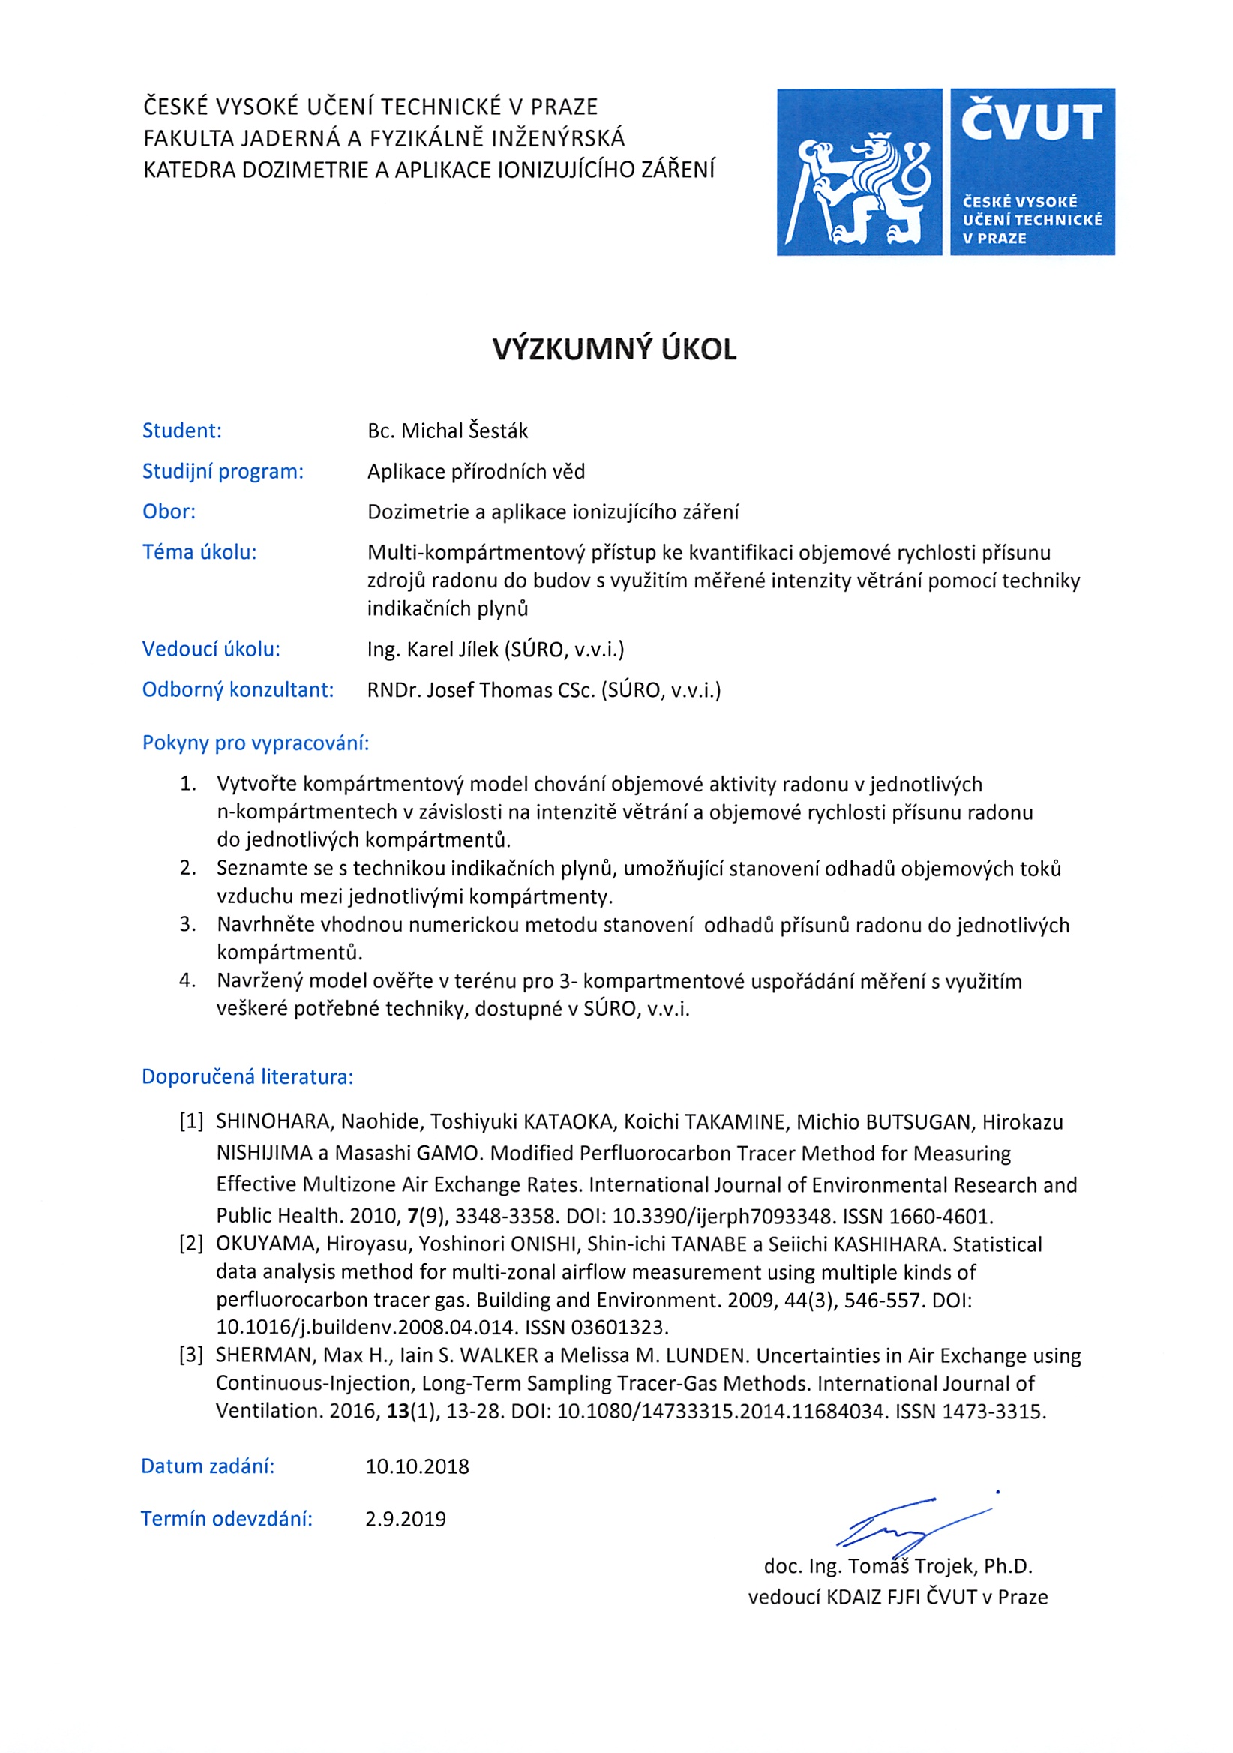
\includepdf[pages={1}]{zadani.pdf}
\newpage
\vspace*{\fill}
\section*{Prohlášení}
Prohlašuji, že jsem svůj výzkumný úkol vypracoval samostatně a použil jsem pouze podklady uvedené v přiloženém seznamu.\\[10pt]
V Praze dne \\[10pt]
\newpage
\vspace*{\fill}
\section*{Poděkování}
Velmi děkuji panu Ing. Karlu Jílkovi za vedení mé práce. Také děkuji panu RNDr. Josefu Thomasovi, Csc. za přečtení a posouzení mé práce. Dále děkuji všem, kdo byli ochotni se se mnou o mém výzkumném úkolu bavit a odpovídat na mé dotazy. 
\newpage
\begin{tabularx}{\textwidth}{>{\itshape}l X}
  Název práce: & \textbf{Multi-kompártmentový přístup ke kvantifikaci  objemové rychlosti přísunu zdrojů radonu do budov s využitím měřené intenzity větrání pomocí techniky indikačních plynů}\\
  Autor: & Bc. Michal Šesták\\
  Obor: & Dozimetrie a aplikace ionizujícího záření\\
  Druh práce: & Výzkumný úkol\\
  Vedoucí práce: & Ing. Karel Jílek\\ 
               & Státní ústav radiační ochrana, v. v. i.\\
  Abstrakt: & Radon v domech představuje vážné zdravotní riziko, a proto je potřeba ho monitorovat a chránit se před ním. Někdy je však těžké určit, odkud radon do domu proniká. Z tohoto důvodu se zavádí veličina objemový přísun radonu zdrojů radonu. Dům, či jiná zájmová stavba se rozdělí na několik kompartmentů, a poté se pomocí měření objemové koncentrace radonu (OAR) a ventilace objektu určí přísuny radonu do těchto kompartmentů. V této práci jsou nejprve uvedeny metody měření OAR a ventilace, následuje odvození výpočetního modelu přísunů radonu. V praktické části byl výpočetní model ověřen na poskytnutých naměřených datech a dále byla provedena tři měření k vyzkoušení a ověření celého procesu. Ukázalo se, že uvedený postup je velmi náchylný na vznik nejistot a tudíž
  je nutné provádět veškerá měření precizně.\\
  Klíčová slova: & radon, kontinuální měření radonu, měření ventilace, indikační plyny, objemové přísuny radonu, python  
\end{tabularx}
\newpage
\begin{tabularx}{\textwidth}{>{\itshape}l X}
  Title: & \textbf{The multi-compartment approach for the quantification of volumetric radon entry rate to buildings using the ventilation intensity measured by a passive multi tracer gas method}\\
  Author: & Bc. Michal Šesták\\
  Abstract: & Radon in buildings represents serious health risk and therefore it should be monitored and there should be some protective remedies against it. However, sometimes it is difficult to locate the radon's sources inside the building. For this purpose the idea of radon entry rate is introduced. The building is divided into several compartments and then the radon entry rates into these compartments are determined from the measurement of the radon volume activities (concentrations) in the compartments and from the measurement of building's ventilation intensity. 

      Firstly the methods of radon concentration measurement and ventilation measurement are introduced in this work. Next, the model for radon entry rates calculation is built. In practical part this model is verified on the provided values of the radon concentrations and the ventilations of several building. Moreover, three full measurements were done. It was found out that the measuring have to be done with big care, otherwise the uncertainties would be huge.\\
  Key words: & radon, continuous radon measurement, ventilation measurement, tracer gases, volumetric radon entries, python 
\end{tabularx}
\newpage 
